\documentclass[border=4pt]{standalone}
% Shared typography and colours for the standalone figures.
\usepackage{unicode-math}
\setmainfont{TeX Gyre Termes}
\setmathfont{TeX Gyre Termes Math}
\usepackage{tikz}
\usetikzlibrary{arrows.meta,positioning,calc,decorations.pathreplacing}
\usepackage{pgfplots}
\pgfplotsset{compat=1.18}

% One colour per element or subsystem. Record the mapping in
% the working repository conventions and use it identically in every figure.
\definecolor{elemA}{HTML}{1F5FA8}
\definecolor{elemB}{HTML}{B8461B}
\definecolor{elemC}{HTML}{2E7D32}
\definecolor{elemD}{HTML}{6A4C93}
\definecolor{frameline}{HTML}{555555}

\begin{document}
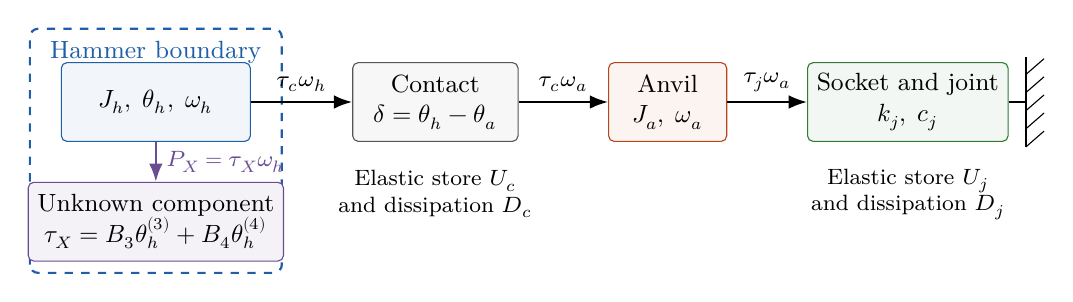
\begin{tikzpicture}[>=Latex,font=\small,box/.style={draw,rounded corners=2pt,minimum height=10mm,align=center}]
\draw[elemA,dashed,thick,rounded corners=3pt] (0,-1.05) rectangle (3.2,2.05);
\node[elemA,anchor=north] at (1.6,2.02) {Hammer boundary};
\node[box,draw=elemA,fill=elemA!6,minimum width=2.4cm] (h) at (1.6,1.12) {$J_h,\;\theta_h,\;\omega_h$};
\node[box,draw=elemD,fill=elemD!7,minimum width=2.4cm] (x) at (1.6,-.40) {Unknown component\\$\tau_X=B_3\theta_h^{(3)}+B_4\theta_h^{(4)}$};
\draw[->,elemD,thick] (h.south)--node[right,font=\footnotesize] {$P_X=\tau_X\omega_h$} (x.north);
\node[box,draw=frameline,fill=black!3,minimum width=2.1cm] (c) at (5.15,1.12) {Contact\\$\delta=\theta_h-\theta_a$};
\node[box,draw=elemB,fill=elemB!6,minimum width=1.5cm] (a) at (8.10,1.12) {Anvil\\$J_a,\;\omega_a$};
\node[box,draw=elemC,fill=elemC!6,minimum width=2.05cm] (j) at (11.15,1.12) {Socket and joint\\$k_j,\;c_j$};
\draw[->,thick] (h.east)--node[above,font=\footnotesize] {$\tau_c\omega_h$} (c.west);
\draw[->,thick] (c.east)--node[above,font=\footnotesize] {$\tau_c\omega_a$} (a.west);
\draw[->,thick] (a.east)--node[above,font=\footnotesize] {$\tau_j\omega_a$} (j.west);
\draw[thick] (j.east)--(12.65,1.12);
\draw[thick] (12.65,.55)--(12.65,1.69);
\foreach \y in {.55,.78,1.01,1.24,1.47} \draw (12.65,\y)--(12.88,\y+.20);
\node[font=\footnotesize,align=center] at (5.15,-.05) {Elastic store $U_c$\\and dissipation $D_c$};
\node[font=\footnotesize,align=center] at (11.15,-.05) {Elastic store $U_j$\\and dissipation $D_j$};
\end{tikzpicture}
\end{document}
